%		PSAR - Sujet 7
%	INTERFACE GRAPHIQUE POUR LA LOGIQUE
%	Sandra Laduranti et Bastien Rigault
%
%	TeX file pour le cahier des charges

\documentclass{article}

\usepackage[utf8]{inputenc}
\usepackage[T1]{fontenc}
\usepackage[french]{babel}
\usepackage{amsmath, amsthm, amssymb}

\usepackage{amsfonts}
\usepackage{gastex}
\usepackage[dvips]{graphics}
\usepackage{pstricks}
\usepackage{a4wide}
\usepackage{multicol}
\usepackage{pst-tree}
\usepackage{tikz-qtree}
\usepackage{color}
\usepackage{array}

\usepackage{tikz}
\usetikzlibrary{arrows}
\tikzstyle{ent}=[circle,draw,thick,inner sep=0pt,minimum size=2.5mm]
\usetikzlibrary{arrows,automata,positioning}
\usetikzlibrary{automata,patterns,topaths,shapes,calc}
\tikzstyle{every picture}+=[>=stealth',initial text=]
\tikzstyle{state}=[rectangle,draw=black]

\definecolor{OliveGreen}{rgb}{0,0.6,0}

\newcommand{\Q}{\mathbb{Q}}
\newcommand{\R}{\mathbb{R}}
\newcommand{\N}{\mathbb{N}}
\newcommand{\Z}{\mathbb{Z}}
\newcommand{\T}{\mathbb{T}}
\newcommand{\Bo}{\mathbb{B}}

\newcommand{\Au}{\mathcal{A}}
\newcommand{\B}{\mathcal{B}}
\newcommand{\C}{\mathcal{C}}
\newcommand{\D}{\mathcal{D}}
\newcommand{\F}{\mathcal{F}}
\newcommand{\G}{\mathcal{G}}
\newcommand{\K}{\mathcal{K}}
\newcommand{\Hr}{\mathcal{H}}
\newcommand{\I}{\mathcal{I}}
\newcommand{\La}{\mathcal{L}}
\newcommand{\M}{\mathcal{M}}
\newcommand{\Net}{\mathcal{N}}
\newcommand{\Pa}{\mathcal{P}}
\newcommand{\Rel}{\mathcal{R}}
\newcommand{\Sy}{\mathcal{S}}
\newcommand{\Ts}{\mathcal{T}}
\newcommand{\X}{\mathcal{X}}

\newcommand{\rel}{\bowtie}
\newcommand{\tr}{\xrightarrow}
\newcommand{\opeq}{\leftrightarrow}
\newcommand{\fee}{\varphi}
\newcommand{\eps}{\varepsilon}
\newcommand{\vect}[1]{\mathbf{#1}}
\newcommand{\fut}{\overrightarrow}
\newcommand\sui[1][a]{\ensuremath{\left(#1_n\right)_{n\in \N}}}

\newcommand{\E}{\textsf{E}}
\newcommand{\A}{\textsf{A}}

\DeclareMathOperator{\cla}{cl}

\theoremstyle{plain}

\newtheorem{theorem}{Théorème}
\newtheorem{lemma}[theorem]{Lemme}
\newtheorem{corollary}[theorem]{Corollaire}
\newtheorem{proposition}[theorem]{Proposition}

\newtheorem{definition}[theorem]{Définition}

\theoremstyle{remark}
\newtheorem{remark}[theorem]{Remarque}
\newtheorem{example}[theorem]{Exemple}

\begin{document}

% PAGE 1
\noindent UPMC, 4I408 \hfill Année 2015--2016 \\
\hfill Sandra Laduranti \\ Bastien Rigault

\begin{center}
	\vspace{4cm}
 	{ \LARGE \bf
 	Projet SAR \\  Une interface graphique pour la logique 
	\\ \vspace{1cm}
 	Cahier des charges
 	}
\end{center}
\clearpage

%PAGE 2
\section{Description du projet}
L'objectif de ce projet, réalisé dans le cadre de l'UE PSAR (4I408)
est de concevoir un logiciel pédagogique pour l'apprentissage de la
logique du premier ordre. Ce logiciel apportera notamment un support
visuel sous la forme d'un jardin et de fleurs permettant d'appréhender
plus facilement les formules de la logique. Les étudiants auront à
leur disposition deux fenêtres : l'une permettant de concevoir un
jardin en y positionnant des fleurs et l'autre permettant d'écrire des
formules à l'aide d'un clavier visuel. Ils pourront alors soit
construire un jardin respectant un ensemble de formule données, ou au
contraire établir des formules à partir d'un jardin donné. Les
formules pourront être analysées de manière automatique afin de
vérifier leur cohérence. Enfin, les étudiants pourront sauvegarder
leurs jardins et leurs formules pour les réutiliser ultérieurement.
\newline La première partie de ce cahier des charges présente d'abord
succinctement la syntaxe de la logique du premier ordre mise en
jeu. La section suivante définit les fonctionnalités principales du
logiciel ainsi que les outils nécessaires à sa réalisation. Enfin les
deux dernières parties concernent l'organisation et la répartition du
travail ainsi que des éventuelles fonctionnalités optionnelles.

\subsection{Logique du premier ordre}
\subsubsection{Les bases de la logique}
Une formule de la logique des prédicats telle qu'elle sera écrite par
les étudiants est constituée de termes, de prédicats, de
quantificateurs et de connecteurs logiques. Prenons par exemple la
formule suivante :

\begin{center}
	$ \forall x Rose(x) \Rightarrow estRouge(x) $
\end{center}

Pour écrire une telle formule, l'étudiant utilise des termes comme
briques de base. Ces termes correspondent soit à l'ensemble $F_0=\{a,
b, ..., t\}$ des constantes, soit à l'ensemble $X=\{v, w, x, y, z\}$
des variables.  \newline Ensuite, il dispose également d'un ensemble
de prédicat $P_i$ d'arité $i$, pour $i\in \{1,2,3\}$. Chaque prédicat
de $P_1, P_2, P_3$ prend ainsi respectivement 1, 2 ou 3 termes en
argument. Dans notre exemple, $Rose(x)$ et $estRouge(x)$ sont deux
prédicats de $P_1$ et prennent la variable $x$ en argument.  \newline
\`A partir de ces formules de base, l'ensemble des formules est défini
inductivement : si $\varphi$ est une formule alors $\lnot \varphi$ est
également une formule. De même si $\varphi_1$ et $\varphi_2$ sont des
formules alors $\varphi_1 \land \varphi_2$, $\varphi_1 \lor \varphi_2$
et $\varphi_1 \Rightarrow \varphi_2$ aussi.  Enfin, si $x \in X$ et
$\varphi$ est une formule alors $\forall x \varphi$ et $\exists x
\varphi$ aussi.  \newline Ce projet utilise un ensemble de prédicat
prédéfinis que l'on regroupera par arité :
\begin{itemize}
	\item[\textit{Unaire}] définissant l'état d'une fleur, elle peut être :
		\begin{itemize}
			\item une rose, une paquette ou une tulipe
			\item petite, moyenne ou grande
			\item rouge, rose ou blanche
			\item à l'est, à l'ouest, au sud ou au nord
		\end{itemize}
              \item[\textit{Binaire}] définissant une relation entre 2
                fleurs, la fleur $a$ peut être :
		\begin{itemize}
                \item à l'est, à l'ouest, au sud ou au nord de la
                  fleur $b$
			\item à la même latitude ou longitude que la fleur $b$
			\item plus grande, plus petite ou de même
                          taille que la fleur $b$
			\item de la même couleur que la fleur $b$
		\end{itemize}
              \item[\textit{Ternaire}] définissant une relation entre
                3 fleurs, la fleur $c$ peut être :
		\begin{itemize}
                \item entre la fleur $a$ et la fleur $b$
		\end{itemize}
\end{itemize}

La section suivante présente quelques exemples de formule utilisant
différents prédicats.

\subsection{Exemple}

On peut par exemple écrire les huit formules ci-dessous.
\begin{itemize}
    \item [(f1)] $d$ est une rose : Rose($d$)
    \item [(f2)] Toutes les fleurs sont des roses : $\forall x Rose(x)$
    \item [(f3)] Il existe une rose : $\exists x Rose(x)$
    \item [(f4)] Toute fleur blanche est plus petite qu'au moins une fleur située à son est :\\
      $\forall x (est\_blanc(x) \Rightarrow \exists y
      (plus\_petit\_que(x, y) \wedge a\_l\_est\_de(y, x)))$
    \item [(f5)] Toute fleur est à l'est, ou à l'ouest, ou au sud, ou au nord : \\
$\forall x (a\_l\_est(x) \vee a\_l\_ouest(x) \vee au\_sud(x) \vee au\_nord(x))$
    \item [(f6)] Toutes les grandes fleurs sont rouges et il n'existe pas de fleur blanche au sud d'une fleur rouge : \\
    $\forall x (est\_grand(x) \Rightarrow est\_rouge(x))\, \wedge \,\neg \exists x (est\_blanc(x) \wedge \exists y (est\_rouge(y) \wedge au\_sud\_de(x, y)))$
    \item [(f7)] Il existe une fleur rouge au nord de la fleur $g : \exists x (est\_rouge(x) \wedge au\_nord\_de(x, g))$
    \item [(f8)] Il existe une unique rose rouge : \\
    $\exists x ((Rose(x) \wedge est\_rouge(x)) \wedge (\forall y (Rose(y) \wedge est\_rouge(y)) \Rightarrow x \circeq y))$
\end{itemize}


\section{Fonctionnalités principales}
\subsection{Le jardin}
\begin{figure}[!h]
\begin{center}
\begin{tikzpicture}[scale=0.375]
\node (n0)    at (-9.5,0)      {Ouest};
\node (n0)    at (9,0)      {Est};
\node (n0)    at (0,-9)      {Sud};
\node (n0)    at (0,9)      {Nord};

\node (n0)    at (0,1)      {$\bullet$};
\node (n0)    at (0,3)      {$\bullet$};
\node (n0)    at (0,5)      {$\bullet$};
\node (n0)    at (0,7)      {$\bullet$};
\node (n0)    at (0,-1)      {$\bullet$};
\node (n0)    at (0,-3)      {$\bullet$};
\node (n0)    at (0,-5)      {$\bullet$};
\node (n0)    at (0,-7)      {$\bullet$};

\node (n0)    at (1,0)      {$\bullet$};
\node (n0)    at (3,0)      {$\bullet$};
\node (n0)    at (5,0)      {$\bullet$};
\node (n0)    at (7,0)      {$\bullet$};
\node (n0)    at (-1,0)      {$\bullet$};
\node (n0)    at (-3,0)      {$\bullet$};
\node (n0)    at (-5,0)      {$\bullet$};
\node (n0)    at (-7,0)      {$\bullet$};

\node (n0)    at (1,2)      {$\bullet$};
\node (n0)    at (1,4)      {$\bullet$};
\node (n0)    at (1,6)      {$\bullet$};
\node (n0)    at (1,-2)      {$\bullet$};
\node (n0)    at (1,-4)      {$\bullet$};
\node (n0)    at (1,-6)      {$\bullet$};
\node (n0)    at (-1,2)      {$\bullet$};
\node (n0)    at (-1,4)      {$\bullet$};
\node (n0)    at (-1,6)      {$\bullet$};
\node (n0)    at (-1,-2)      {$\bullet$};
\node (n0)    at (-1,-4)      {$\bullet$};
\node (n0)    at (-1,-6)      {$\bullet$};

\node (n0)    at (2,1)      {$\bullet$};
\node (n0)    at (2,3)      {$\bullet$};
\node (n0)    at (2,5)      {$\bullet$};
\node (n0)    at (2,-1)      {$\bullet$};
\node (n0)    at (2,-3)      {$\bullet$};
\node (n0)    at (2,-5)      {$\bullet$};
\node (n0)    at (-2,1)      {$\bullet$};
\node (n0)    at (-2,3)      {$\bullet$};
\node (n0)    at (-2,5)      {$\bullet$};
\node (n0)    at (-2,-1)      {$\bullet$};
\node (n0)    at (-2,-3)      {$\bullet$};
\node (n0)    at (-2,-5)      {$\bullet$};

\node (n0)    at (3,0)      {$\bullet$};
\node (n0)    at (3,2)      {$\bullet$};
\node (n0)    at (3,4)      {$\bullet$};
\node (n0)    at (3,-2)      {$\bullet$};
\node (n0)    at (3,-4)      {$\bullet$};
\node (n0)    at (-3,0)      {$\bullet$};
\node (n0)    at (-3,2)      {$\bullet$};
\node (n0)    at (-3,4)      {$\bullet$};
\node (n0)    at (-3,-2)      {$\bullet$};
\node (n0)    at (-3,-4)      {$\bullet$};

\node (n0)    at (4,1)      {$\bullet$};
\node (n0)    at (4,3)      {$\bullet$};
\node (n0)    at (4,-1)      {$\bullet$};
\node (n0)    at (4,-3)      {$\bullet$};
\node (n0)    at (-4,1)      {$\bullet$};
\node (n0)    at (-4,3)      {$\bullet$};
\node (n0)    at (-4,-1)      {$\bullet$};
\node (n0)    at (-4,-3)      {$\bullet$};

\node (n0)    at (5,0)      {$\bullet$};
\node (n0)    at (5,2)      {$\bullet$};
\node (n0)    at (5,-2)      {$\bullet$};
\node (n0)    at (-5,0)      {$\bullet$};
\node (n0)    at (-5,2)      {$\bullet$};
\node (n0)    at (-5,-2)      {$\bullet$};

\node (n0)    at (6,1)      {$\bullet$};
\node (n0)    at (-6,1)      {$\bullet$};
\node (n0)    at (6,-1)      {$\bullet$};
\node (n0)    at (-6,-1)      {$\bullet$};

%\draw[dotted] (-8,8) --  (-8,-8);
\draw[dotted] (-7,8) --  (-7,-8);
\draw[dotted] (-6,8) --  (-6,-8);
\draw[dotted] (-5,8) --  (-5,-8);
\draw[dotted] (-4,8) --  (-4,-8);
\draw[dotted] (-3,8) --  (-3,-8);
\draw[dotted] (-2,8) --  (-2,-8);
\draw[dotted] (-1,8) --  (-1,-8);
\draw[->] (0,-8) --  (0,8);
\draw[dotted] (1,8) --  (1,-8);
\draw[dotted] (2,8) --  (2,-8);
\draw[dotted] (3,8) --  (3,-8);
\draw[dotted] (4,8) --  (4,-8);
\draw[dotted] (5,8) --  (5,-8);
\draw[dotted] (6,8) --  (6,-8);
\draw[dotted] (7,8) --  (7,-8);
%\draw[dotted] (8,8) --  (8,-8);

%\draw[dotted] (-8,8) --  (8,8);
\draw[dotted] (-8,7) --  (8,7);
\draw[dotted] (-8,6) --  (8,6);
\draw[dotted] (-8,5) --  (8,5);
\draw[dotted] (-8,4) --  (8,4);
\draw[dotted] (-8,3) --  (8,3);
\draw[dotted] (-8,2) --  (8,2);
\draw[dotted] (-8,1) --  (8,1);
\draw[->] (-8,0) --  (8,0);
\draw[dotted] (-8,-1) --  (8,-1);
\draw[dotted] (-8,-2) --  (8,-2);
\draw[dotted] (-8,-3) --  (8,-3);
\draw[dotted] (-8,-4) --  (8,-4);
\draw[dotted] (-8,-5) --  (8,-5);
\draw[dotted] (-8,-6) --  (8,-6);
\draw[dotted] (-8,-7) --  (8,-7);
%\draw[dotted] (-8,-8) --  (8,-8);

\draw[densely dashed] (0,0) -- (7,7);
\draw[densely dashed] (0,0) -- (-7,-7);
\draw[densely dashed] (0,0) -- (7,-7);
\draw[densely dashed] (0,0) -- (-7,7);
\end{tikzpicture}
\end{center}
\caption{Places d'un jardin}\label{lagrille}
\end{figure}

Les termes considérés dans le projet désignent des fleurs positionnées
sur une grille. La figure 1 représente la grille : les points noirs
symbolisent les places où peuvent être disposées les fleurs (il y a au
plus une fleur par place). Chaque place est identifiée par ses
coordonnées (le point $(0,0)$ est au centre de la grille). L'ensemble
des places possibles est donc :

\[
\mathrm{Places}  = \left \{
\begin{array}{c}
(0,7) ,
\\
(-1,6), (1,6) ,
\\
(-2,5) , (0,5) , (2,5),
\\
(-3,4) , (-1,4) , (1,4) , (3,4),
\\
(-4,3), (-2,3), (0,3) , (2,3), (4,3),
\\
(-5,2),(-3,2) , (-1,2) , (1,2) , (3,2), (5,2),
\\
(-6,1),(-4,1), (-2,1), (0,1) , (2,1) , (4,1),(6,1),
\\
(-7,0) , (-5,0) , (-3,0) , (-1,0) , (1,0) , (3,0) , (5,0) , (7,0) ,
\\
(-6,-1),(-4,-1), (-2,-1), (0,-1) , (2,-1), (4,-1),(6,-1),
\\
(-5,-2),(-3,-2), (-1,-2), (1,-2) , (3,-2),(5,-2),
\\
(-4,-3), (-2,-3) , (0,-3) , (2,-3), (4,-3),
\\
(-3,-4), (-1,-4), (1,-4) , (3,-4) ,
\\
(-2,-5) , (0,-5) , (2,-5),
\\
(-1,-6),  (1,-6),
\\
(0,-7)
\\
\end{array}
\right \}
\]

Chaque fleur appartient à une espèce (les roses, les pâquerettes et
les tulipes), est d'une certaine taille (grande, moyenne ou petite) et
d'une certaine couleur (rouge, rose, blanche).

 \[ \begin{array}{l}
   Especes =  \{rose, paquerette,tulipe \}, \\
   Tailles =  \{grand, moyen, petit \},\\
   Couleurs = \{rouge,rose, blanc \}.
\end{array}
\]

Certaines fleurs ont un nom : il s'agit d'une constante de $F_0$ (deux
fleurs différentes ne peuvent pas avoir le même nom). Un jardin $j$
est la donnée d'une grille sur laquelle sont disposées des fleurs
(chaque jardin contient au moins une fleur) et est représentée par une
liste de quintuplets. Chaque quintuplet $((x, y), e, t, c, n) \in j$
est un élément du produit cartésien :

 \begin{center}
 $Places \times Especes \times Tailles \times Couleurs \times(F_0 \cup \left \{None\right \})$ 
 \end{center}
 
\noindent
et exprime qu'une fleur de nom $n$ ($n$ = None si la fleur n'a pas de
nom), d'espèce $e$, de taille $t$ et de couleur $c$ se trouve à la
place $(x, y)$ dans le jardin j. L'ensemble des jardins possibles est
donc :
 
  \begin{center}
  $J = \wp(Places \times Especes \times Tailles \times Couleurs \times(F_0 \cup \left \{None\right \})\setminus\left \{\emptyset\right \}$ 
 \end{center}
 
\subsection{Exemples de formules}

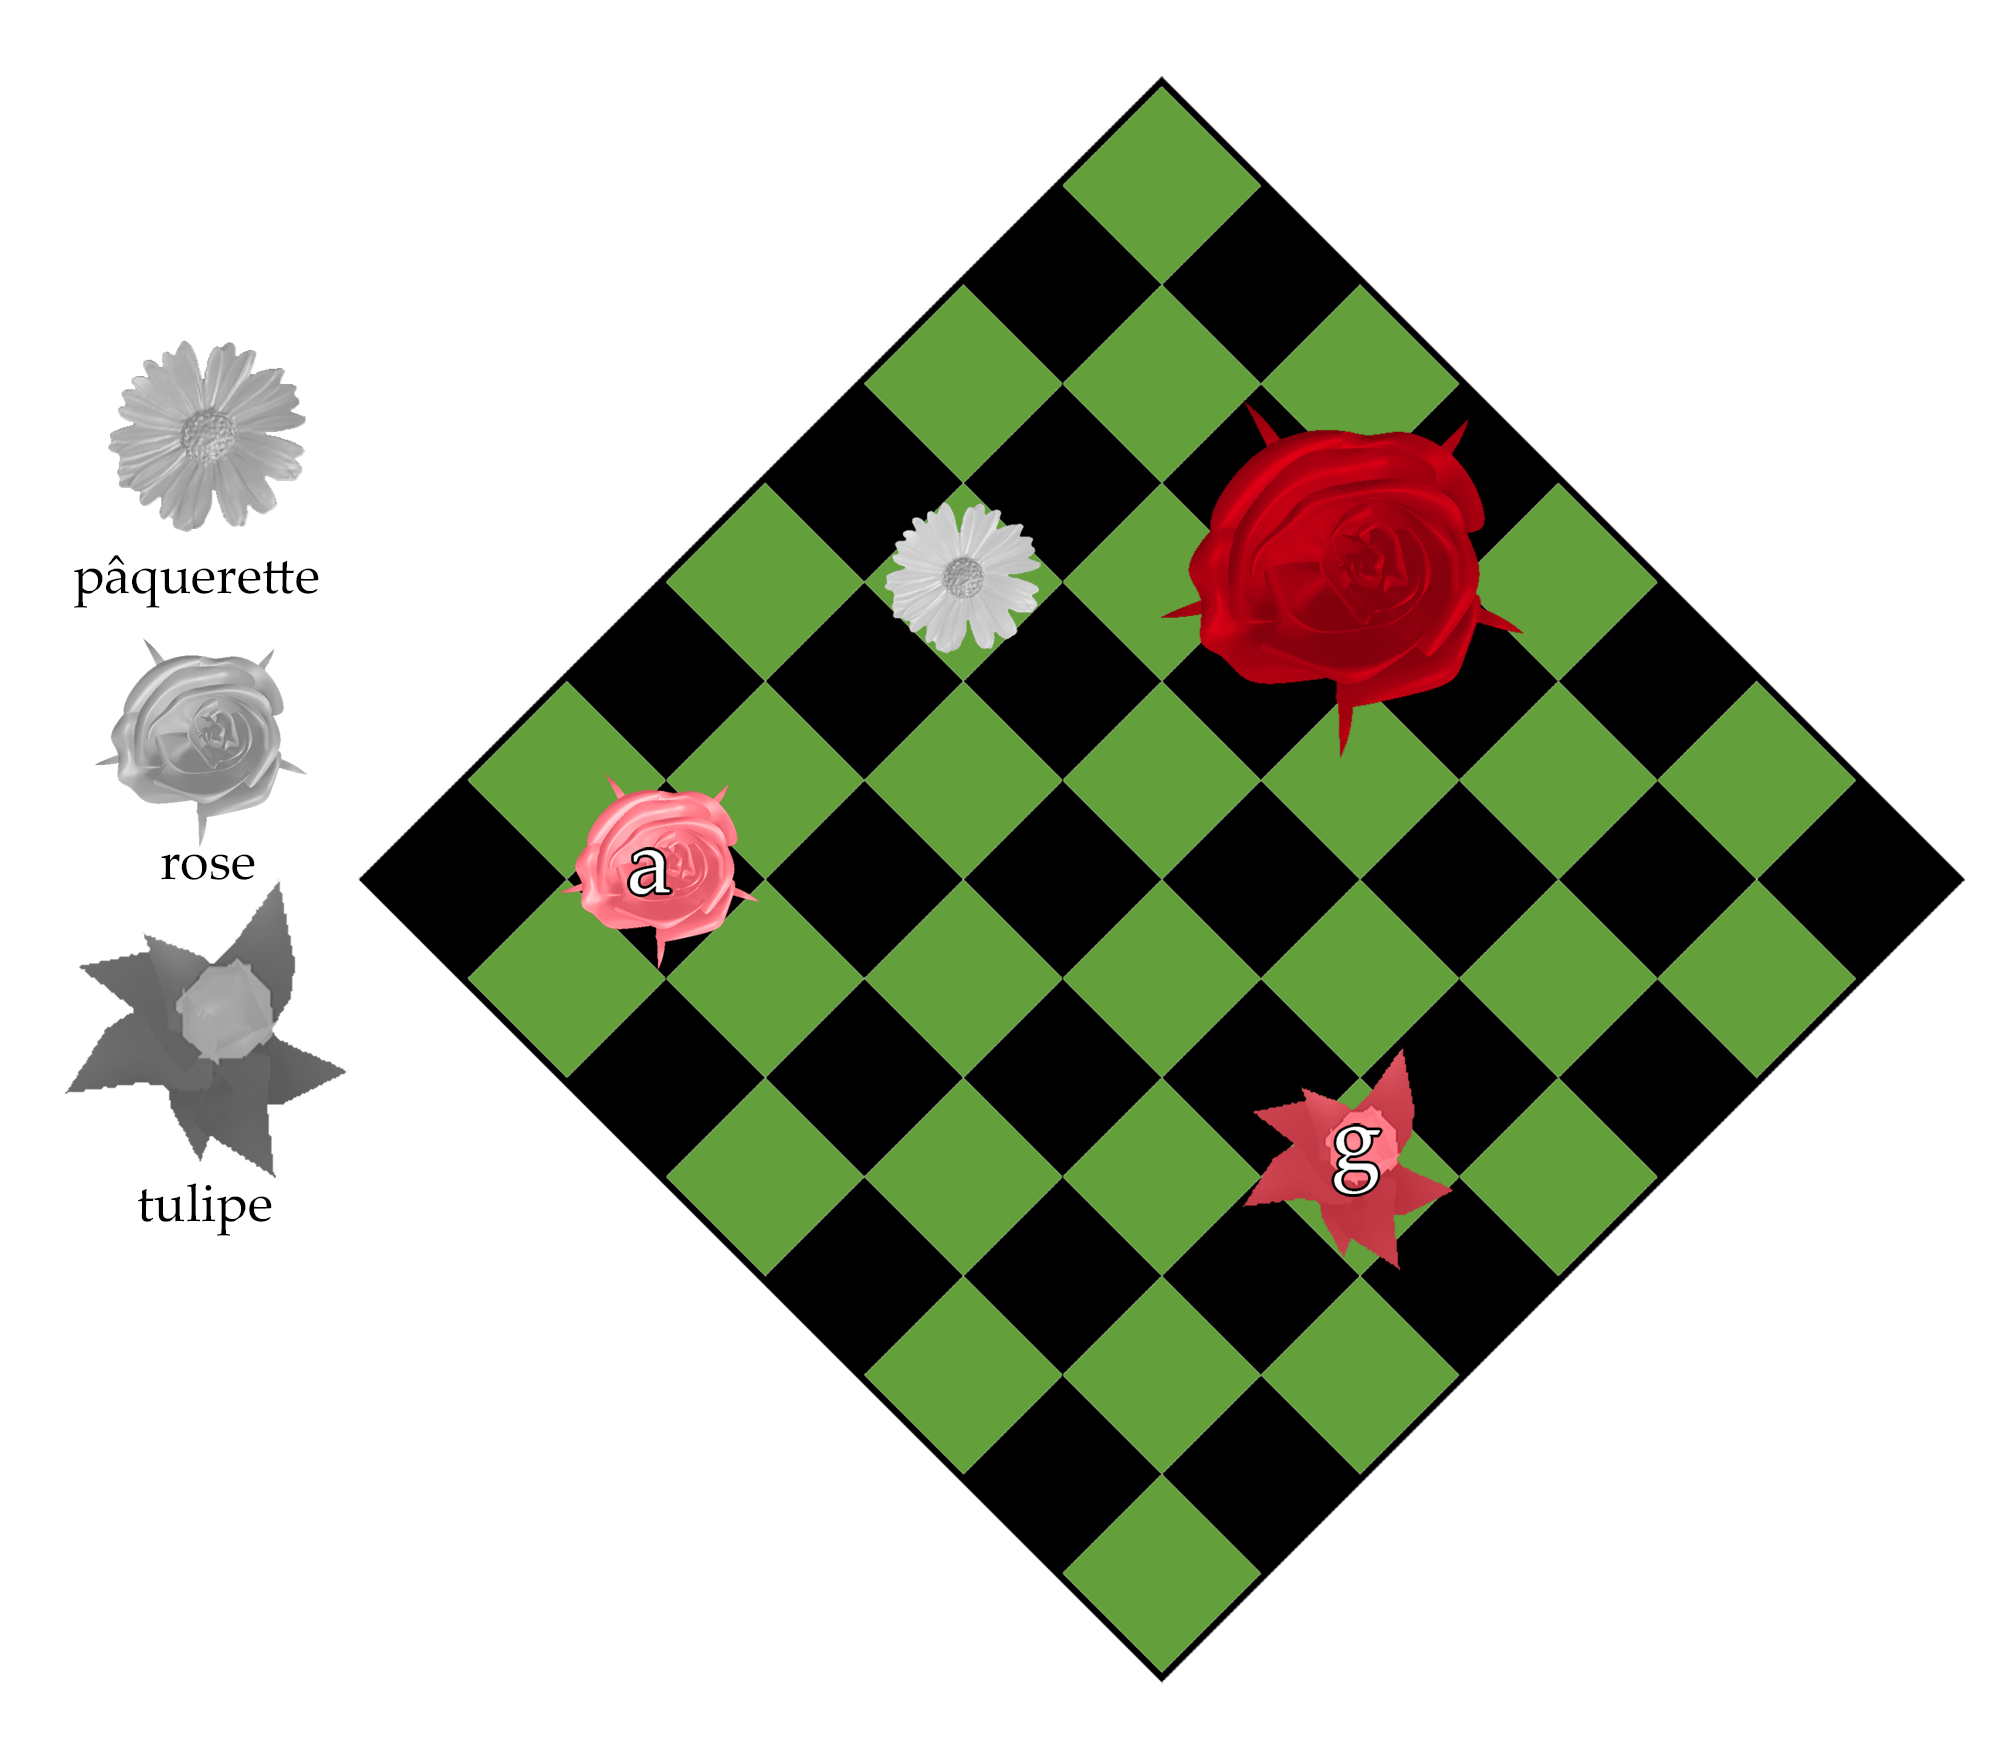
\includegraphics{formulesDemo} ;
Voici quelques exemples de formules dans le jardin ci-dessus:

\begin{itemize}
    \item [(f1): {\color{red} FAUX}] Toutes les fleurs sont des roses : $\forall x Rose(x)$
    \item [(f2): {\color{OliveGreen} VRAI}] Il existe une rose : $\exists x Rose(x)$
    \item [(f3): {\color{OliveGreen} VRAI}] Toute fleur blanche est plus petite qu'au moins une fleur située à son est : \\
$\forall x (est\_blanc(x) \Rightarrow \exists y  (plus\_petit\_que(x, y) \wedge a\_l\_est\_de(y, x)))$
	\item [(f4): {\color{red} FAUX}] Toutes les tulipes sont rouges: $\forall x Tulipe(x) \Rightarrow estRouge(x)$
    \item [(f5): {\color{OliveGreen} VRAI}] Toutes les grandes fleurs sont rouges et il n'existe pas de fleur blanche au sud d'une fleur rouge : \\
    $\forall x (est\_grand(x) \Rightarrow est\_rouge(x))\, \wedge \,\neg \exists x (est\_blanc(x) \wedge \exists y (est\_rouge(y) \wedge au\_sud\_de(x, y)))$
    \item [(f6): {\color{red} FAUX}] $a$ est une pâquerette : $Paquerette(a)$

    \item [(f7): {\color{OliveGreen} VRAI}] Il existe une fleur rouge au nord de la fleur $g : \exists x (est\_rouge(x) \wedge au\_nord\_de(x, g))$
    \item [(f8): {\color{OliveGreen} VRAI}] Il existe une unique rose rouge : \\
    $\exists x ((Rose(x) \wedge est rouge(x)) \wedge (\forall y (Rose(y) \wedge est\_rouge(y)) \Rightarrow x \circeq y))$
\end{itemize}

\subsection{Aspect graphique}
\subsubsection{En résumé}
Les éléments nécessaires sont :
\begin{itemize}
	\item un jardin représenté par une grille de taille fixe,
	\item des fleurs pouvant être disposées sur le jardin et ayant
          un visuel différent selon leurs espèces, tailles et
          couleurs,
	\item un menu permettant de positionner de nouvelles fleurs à
          la souris et d'en changer l'aspect,
	\item un menu permettant d'écrire et vérifier des formules de
          la logique du premier ordre à l'aide d'un clavier virtuel et
          d'une liste de 5 variables et de 20 constantes,
	\item un menu permettant de sélectionner une variable ou une
          constante,
	\item un clavier visuel permettant de sélectionner les
          connecteurs de la logique (not, et, ou, pour tout, etc.),
	\item un menu permettant de sauvegarder et de charger des
          jardins et/ou des ensembles de formules.
\end{itemize}

\subsubsection{Simulation de rendu}

\begin{center}
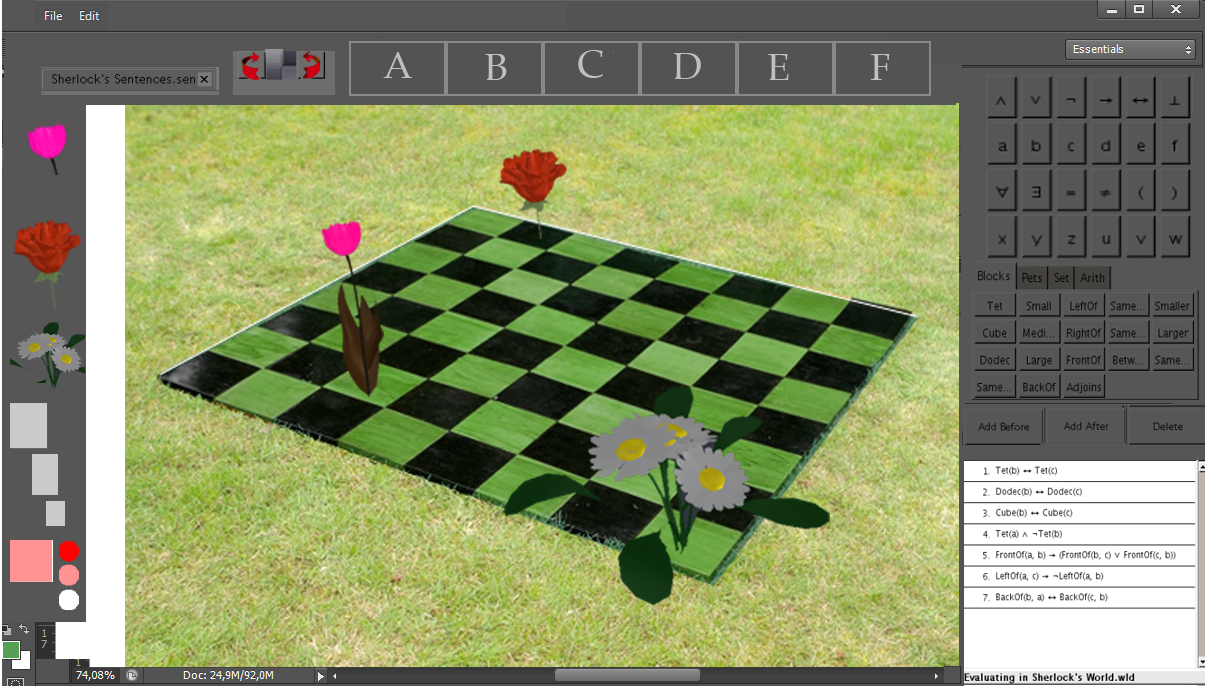
\includegraphics{simulation} ;
\end{center}

\section{Aspects techniques}
\subsection{Analyse syntaxique}

L'analyse syntaxique se fera à l'aide de l'outil Grammatica version
1.6 (libre de droit sous licence BSD). Il s'agit d'un générateur
d'analyseur syntaxique qui, après avoir reçu une grammaire spécifique
en entrée, produit un parseur pour cette grammaire en C\#. Ce code
n'est généré qu'une seule fois et est capable d'analyser des formules
données sous forme de chaînes de caractères. Le résultat final obtenu
est soit un message d'erreur détaillé si la formule est incorrecte
soit un arbre syntaxique représenté en C\# comme l'illustre la figure
suivante :

\begin{center}
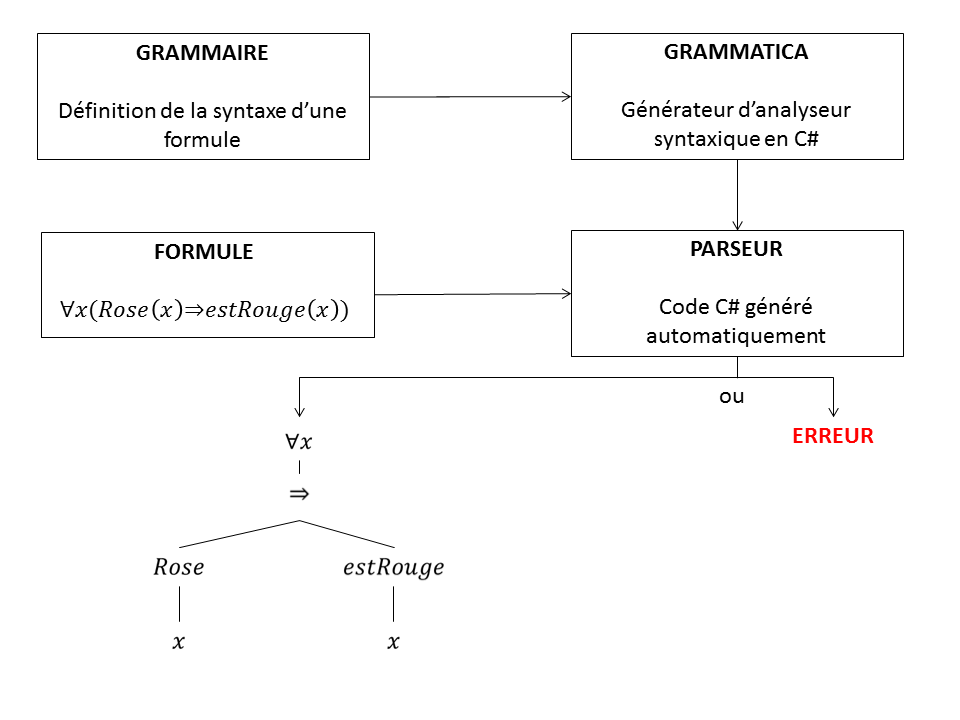
\includegraphics[width=100mm, height=70mm]{syntaxtree} ;
\end{center}

\subsection{Vérification des formules}
La vérification des formules sera réalisée en trois parties
distinctes, à savoir leur récupération, la vérification de leur
intégrité syntaxique (vue au chapitre précédent) et enfin la
vérification de leur validité dans le jardin donné.

\subsubsection{Choix des langages}
Le choix des langages a été régi par la contrainte de communication
entre deux langages de programmation différents. L'outil de
vérification de formules fourni de base étant en Ocaml, le besoin
premier était de trouver comment communiquer avec ce dernier.  En
parallèle il fallait également prendre en compte les contraintes
esthétiques, l'application devant être au final à la fois solide et
conviviale. La solution de la programmation en Java a donc été
immédiatement éliminée par souci de manque d'esthétisme dans ses GUI.

Suite à de nombreuses recherches, le choix s'est donc porté sur du
C\#, offrant un outil de développement permettant de faire le pont
entre Ocaml et C\#.  De plus le choix de C\# a été confortée par la
possibilité d'utiliser ce langage avec le moteur de jeu Unity 5.  Les
avantages de ce moteur étant tout d'abord sa gratuité mais également
son moteur 3D qui entre en parfaite adéquation avec les objectifs
finaux du projet.

\subsubsection{Interprétation des formules}
En premier lieu, l'étudiant entrera dans l'application, à l'aide de sa
souris et sur le clavier optique fourni par le programme, une formule
à valider.  La formule sera alors récupérée via les événements de la
GUI de Unity et seront transmis au module d'analyse syntaxique de
l'application via C\# (vu au chapitre de l'analyse syntaxique). En
supposant que la formule ait passé la vérification syntaxique, elle
sera alors envoyé au vérificateur de formule.

Comme vu précédemment, cette partie a impliqué le choix du langage de
par sa complexité en terme de programmation. Peu de langages
permettent de faire la liaison avec Ocaml. Les formules récupérées
préalablement en C\# seront donc transmises via un "pont" formé par
l'outil CSML. Cette étape nécessite de renvoyer également le jardin
dans son nouvel état, des modifications pouvant être apportées entre
deux formules.

Le vérificateur de formule en Ocaml pourra ensuite vérifier
l'exactitude de la formule dans le contexte donné et renvoyer le
résultat via le pont CSML à l'application en C\# qui remontera alors
graphiquement à l'étudiant la décision de l'application.


\section{Organisation}
\subsection{Outils}
Il a été décidé d'utiliser un gestionnaire de version pour faciliter
l'accès aux documents et le travail en parallèle via des branches de
développement.  Le choix s'est porté sur github qui offre des dépôts
privés aux étudiants.

\subsection{Partage des tâches}
A partir de la date de rendu officielle du cahier des charges de
l'application, il reste 2 mois et demi de programmation à séquencer.
\noindent
Le programme s'axe sur trois grandes parties, deux complexes:
\begin{itemize}
\item analyse syntaxique,
\item liaison Ocaml et C\# avec CSLM,
\end{itemize}
\noindent
et une partie plus simple mais longue:
\begin{itemize}
\item sauvegarde des jardins,
\item programmation de l'interface graphique.
\end{itemize}

Afin de paralléliser au maximum les taches, une personne devra
s'occuper de l'analyse syntaxique pendant que l'autre s'occupera de la
liaison CSML.  Cette partie se déroulera sur un mois et demi de
programmation afin de laisser le temps de faire le plus de tests
possibles. Il est important que cette partie de l'application soit la
plus robuste possible.\\ Le dernier mois sera consacré à toute
l'interface graphique et les différents modules de celle-ci seront
partagés entre les programmeurs:
\begin{itemize}
\item affichage 3D/2D du jardin,
\item création du clavier optique,
\item modélisation des fleurs,
\item création des divers menus.
\end{itemize}
\noindent
Dans le cas où le programme serait entièrement fonctionnel avant la
période impartie, il pourra être envisagé d'ajouter des
fonctionnalités optionnelles.

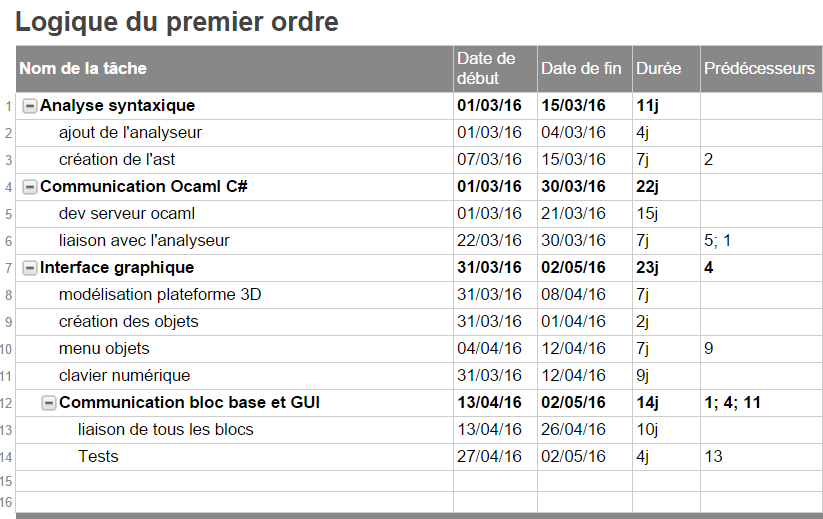
\includegraphics{gantt1} ;
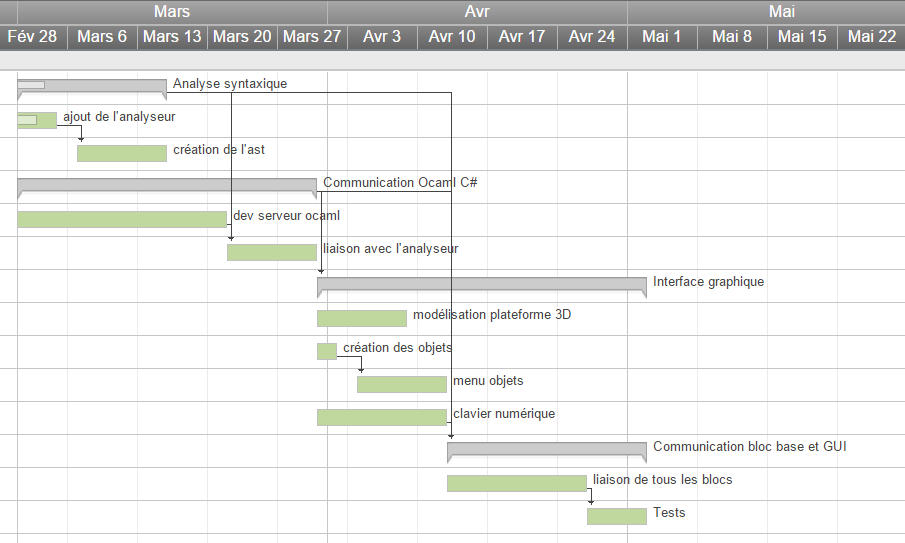
\includegraphics[scale=0.2]{gantt2} ;

\section{Fonctionnalités optionnelles}
\subsection{Aspects graphiques}
\begin{itemize}
\item Animation lors de l'ajout d'une fleur et/ou temps d'inactivité
  de l'utilisateur trop long.
\item Possibilité de saisie de formule au clavier uniquement avec un
  système de raccourci.
\end{itemize}
\subsection{Aspects techniques}
\begin{itemize}
\item Amélioration de l'algorithme de vérification syntaxique des formules
  pour indiquer où se trouve l'erreur.
\item Implémentation d'un système de \og retour en arrière \fg.
\end{itemize}
\end{document}
